\documentclass[twocolumn,prl]{revtex4-1}
\usepackage{graphicx}
\usepackage{amsmath}
\begin{document}
\title{An appropriate title describing a smashing new discovery}
\author{A. Student}
\author{A. Professor}
\affiliation{Brown University}
\begin{abstract}
Here goes the abstract of the paper. We describe how to write PRL's. We conclude that the universe must be doughnut-shaped.
\end{abstract}
\maketitle

Many wise (and many not-so-wise) people have written PRL's, and many of them have written documents about how to write PRL's. Here is my version of the how-to. Feel free to ignore any or all of it. This file can also be used as a template for writing new PRL's.

A paper starts with an introduction to the topic. The introduction to letters, such as one published in Physical Review Letters, is usually short and highlights the background that the research presented in the paper most directly addresses. All relevant literature must be cited in this background, and hence reading all related (or unrelated) papers and understanding them is crucial for writing an introduction. For example, scientists have pondered for ever about the shape of the universe\cite{aurich2004can,ellis2003shape,adams2001shape,gomero2000signature,cornish1998can}.

The discussion then advances to the discoveries claimed in the letter. Be as concise and precise about the claims, because the rest of the letter must provide support for justifying them. Claims can be strong (e.g. we show that the universe is shaped like a doughnut) if one can justify it through suitable evidence. Otherwise claims can be inconclusive, and possibly vague (e.g. our data suggests that the universe may be shaped like a doughnut, or out data is consistent with a doughnut-shaped universe). Vague and inconclusive claims usually do not make good subject matter for papers, hence it is usually a good idea to continue the research and continuously revaluate the possible conclusive claims one can make with the evidence.

Once the claims are made, it is imperitive that one provide evidence supporting and justifying them. This evidence may be in the form of an experiment, a theoretical calculation, a numerical solution, or a combination. To set the stage, the letter continues with a description of the method used to generate the supporting evidence (experimental method, mathematical model, numerical method, etc). The description of these methods needs to be self-contained and complete but brief (because such letters usually have a restriction on the total length). These methods set the stage for discussing acquired data and drawing conclusions. It is a good idea to include a schematic figure describing the experimental setup or mathematical model, like I have shown in figure \ref{fig:Schematic_Doughnut}.

Describe the details data generated as part of the research using the methods described in the previous paragraph(s). The data can take the form of experimentally measured quantities (suitably post-processed to be relevant), numerical solutions, or theoretical analyses or relations. One typically does not draw any conclusions at this stage, but merely describes the ``observations'' from ones analysis or experiments. Such data is also presented in the form on one or more figures. Due to length constraints, one has to choose the data to be presented very carefully; no more than a total of 4 figures can be accommodated within this length. Due to the length restriction, the number of equations one can use in a PRL is also limited (around 10), and one has to be very judicious in the choice of these equations, such as
\begin{equation}
E = m c^2 \quad \text{(Einstein)}, \label{eqn:Einstein}
\end{equation}
where $E$ is energy, $m$ is mass, and $c$ is the speed of light.

If the observations support any claims, they are discussed next. These claims better be exactly the ones mentioned right after the introduction. Argue from the data how the claims are verified. For instance, clearly from \eqref{eqn:Einstein}, the universe is exploding with energy. Doughnuts also have a lot of calories. But a calorie is just a unit for energy. Therefore, the universe must be doughnut shaped.
\begin{figure}[htb]
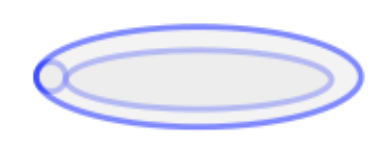
\includegraphics{Figures/Schematic_Doughnut}
\caption{Scientists have long wondered if the universe is doughnut shaped shown above.}
\label{fig:Schematic_Doughnut}
\end{figure}


Conclude the letter by reiterating the main conclusion. Discuss the possible connections with other research in the literature, for example, someone was wondering how the shape of the universe affects legal research process\cite{mills2003shape} (I am not joking, read this reference). This book\cite{oshea2009poincare} also claims the Poincare conjecture has something to do with the shape of the universe. Also discuss any shortcomings. And conclude the paper. 
\bibliography{newfile}
\end{document}
